% !TEX root = ../main.tex
\chapter{Data Collection}\label{chap:experiment}

  \section{Research Strategy}\label{sec:researchStrategy}
    This section will provide information about the chosen research strategy. A research strategy is being considered as the selected strategy for being able to answer the main research goals; the hypotheses and the research questions. Briony J. Oates \cite{empiriske} presents six different research strategies: survey, experiment, design and creation, case study, action research, and ethnography. This section will not go further in describing the difference between the six strategies, but rather explain the choice of research strategy. The detailed work behind the choice in research design was carried out in preliminary work beforehand of this thesis \cite{prosjektoppgave}.

    The selected research strategy for this dissertation is a survey. The idea of a survey is that it will obtain some kind of data from a large group of people or events, in a standardized and systematic way \cite{empiriske}. The survey is chosen due to the amount of data needed for the analysis, as well as the lack of time for choosing other approaches, like interviews and other observation techniques. There are different ways of creating a survey, for example, pen-and-paper or using an online survey. For this research, an online survey is selected for several reasons. First, a pen-and-paper survey is too time-consuming to perform and are not scalable for international data collection. It is also desired to keep responses anonymous due to the topic of research. The form of administration is, therefore, self-administered as there is no one present when the respondent answers the survey. More information about the sampling technique is described in section \ref{sec:samplingTechnique}.

    In the preliminary work, wireframes were created as a draft of the survey. These wireframes can be found in Appendix \ref{ap:wireframes}. Chapter \ref{sec:survey} will have a final implemented version giving a more detailed description of the survey.

  \section{Sampling Technique}\label{sec:samplingTechnique}
    The {\it sampling frame} is a list of the whole population of people that could be included in the survey. When looking at the sample of this study, there is not possible to make a limited sampling frame that can be summered in a list. The population of the sample frame is considered as all people with a smartphone because this research looks at people's choice of Graphical Password, in particular the Android Lock Patterns that is a mobile authentication scheme.

    When conducting a survey, it needs to be decided how to select people from the sampling frame. There are two different ways of doing sampling: probability sampling and non-probability sampling \cite{empiriske}. Probability sampling means that the sample has been chosen because the researcher believes that there is a high probability that the sample of respondents selected is representative for the overall population being studied. Non-probability sampling means that the researcher does not know whether the sample of people is the overall population.

    Because of the broad sampling frame it would be feasible to use non-probability sampling for this research. When using non-probability sampling, we make a decision that it is not practicable to describe a representative sample because there is too much uncertainty about the respondents that will voluntary answer the questionnaire. When choosing a non-probability sampling, we need to select an {\it sampling technique}. The possible sampling techniques we can choose from is purposive sampling, snowball sampling, self-selection sampling, and convenience sampling \cite{empiriske}. The {\it purposive sampling technique} requires the researcher deliberately to choose people that are likely to produce valuable data to meet the purpose of the research. This requirement would not be a good technique because I am not able to pick who would participate, as well as the data collection need to be performed worldwide. A Purposive sampling technique would maybe provide a more uniform collection of people, but it is hard to control respondents when the survey is distributed over the Internet.
    The {\it snowball sampling technique} utilize the network from one person of the sample frame, and then collects new names from that person. The need for directly communicate with respondents is not possible for me as a researcher. {First}, I have no contact with the respondents. {Second}, the respondents, should remain anonymous when answering the questionnaire, as well as there should be possible to track the information back to the respondent. When using the {\it convenience sampling technique}, the researcher only selects respondents who are convenient for them, because they are easy to reach or willing to help.

    When doing {\it self-selection sampling}, the researcher advertises their interest in a particular topic and their need for respondents and collect data from anyone who are willing to participate. The self-selection sampling strategy looks like an excellent fit for the research. The survey needs to be distributed over the Internet, and the self-selection strategy will support this choice. People who select themselves for research often do so because they have strong feeling for the subject, or that the research can bring them a personal benefit. A self-selection sampling technique may also reduce the bias that can be introduced when the researcher hand-picks the respondents. With the self-selection sampling strategy allows all interested peoples with a smartphone to participate in the research. The self-selection is a useful technique when directly contact is not achievable. The self-selection sampling remains the technique that are looking as the best fit for this research.

  \section{Review of Human Properties}\label{sec:reviewofproperties} 

      When using an online survey, the human properties must be carefully selected. {\it First}, when a survey is distributed on the Internet there is no way back, and we need to be sure that the chosen questions will provide sufficiently and relevant data for answering the hypothesis. {\it Second}, we need to review all human properties and only select a suited number of them. A too long survey may result in a small number of responses because the time needed to complete the survey if all the properties is included. {\it Third}, some of the properties may not have a suitable grouping of answers, and may be challenging to include in a survey that needs to be replied to on a mobile device. If such a property is included, it needs to provide irreplaceable and valuable information for the analysis. The survey should try to avoid time-consuming and complicated questions if possible. This section will provide a detailed review of the human properties.

      \subsection*{Age and Gender} 
      A group of people within a particular group of age may have different risk awareness. A person with an age of 30-40 years and a person younger than 20 years may have different concerns with security. A person of age between 30-40 may use their phone to perform a task with requiring high security, like tasks related for work purposes. A person with an age below 20 may not have the same security awareness because of the different use of mobile devices, as well as experience. Age is also interesting demographic information that can be used to group the respondents into distinct subgroups. When looking at gender, psychological studies have reported that males are more likely to take risks than females \cite{Byrnes}. In the literature review, there were no results found related to gender and risk awareness. However, researchers have found bias in the password selection process of {\it PassFace} when looking at gender.

      \subsection*{Language preference}
      By asking the respondent about their language preference it can be used to check whether the alphabet a respondent use impacts their choice in lock pattern. For example, Chinese words are written in a different way then people using the Latin alphabet. In the Android Unlock Patterns, people are able to create patterns looking the same as the letters \texttt{'L'}, \texttt{'M'}, and \texttt{'O'}. The Figure~\ref{fig:letters2} there is an illustration the letters that are possible to select a lock pattern. The same possibility could be found in languages using a different alphabet than the Latin. When looking at PIN codes, there are certain numbers that have a different meaning than only its numeric value. In China, people are associating certain words with numbers or things based on the similarities of sound. For example, the number eight is considered as a lucky number because it is pronounced "ba", which sounds like the Chinese word for prosperity \cite{ChineseChatCodes}. Other numbers like 4 and 775 are pronounced in the same way as "death" and "Kiss me", respectively. Looking at the selection of PIN codes based on people's language, people tend to choose PIN codes that they can associate to a number of special meanings. Examples of this behavior are PIN selection corresponding to date of birth. 

        \begin{figure}[H]
          \centering
          \subfigure[The letter L]{
            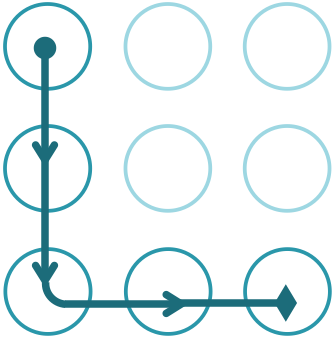
\includegraphics[width=0.25\textwidth]{pics/letters/bokstavenL.png}
          }
          \vspace{0.2cm}
          \subfigure[The letter M]{
            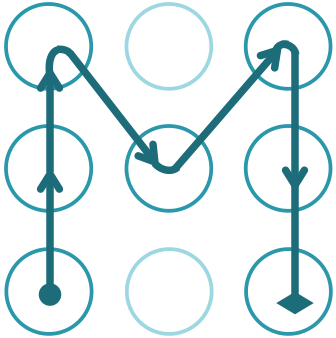
\includegraphics[width=0.25\textwidth]{pics/letters/bokstavenM.png}
          }
          \vspace{0.2cm}
          \subfigure[The letter O]{
            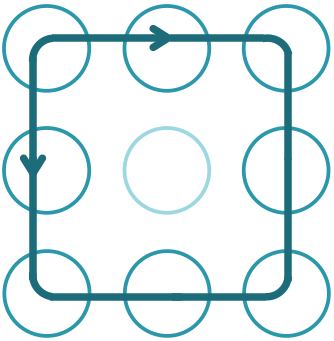
\includegraphics[width=0.25\textwidth]{pics/letters/bokstavenO.png}
          }
          \caption{Patterns corresponding to letters}
          \label{fig:letters2}
        \end{figure}

      \subsection*{Handedness}
      An interesting property of humans is the fact that people write with either left or right hand (and sometimes both). Handedness can influence the way a person are holding a mobile phone, and may impact their choice of lock pattern. In the literature review, it was not found any studies that reported results of people choices in patterns based on handedness. Published research \cite{Uellenbeck} found that over 40\% of the participants in their study started their Android pattern by beginning in the upper-left corner, but did not record the hand used when collecting the patterns. A question to be answered is whether a left-handed person using the left hand while interacting with the screen increases the probability for starting in the upper right corner. Figure \ref{fig:handedness} illustrates handedness and likely starting point as a hypothesis, where the percentages attached to the nodes are indicating the probability for starting in the node. The right part of Figure \ref{fig:handedness} are collected from the research by Uellenbeck \cite{Uellenbeck} while the numbers on left part are only hypothetical numbers. Since it is more likely that people are right-handed, are we able to mirror the results in the right figure for left-handed people? My hypothesis as stated earlier is that people that are left-handed are more likely to start in the upper right corner, while people that are right-handed are more likely to start in the upper left corner.

        \begin{figure}[H]
          \centering
          \subfigure{
            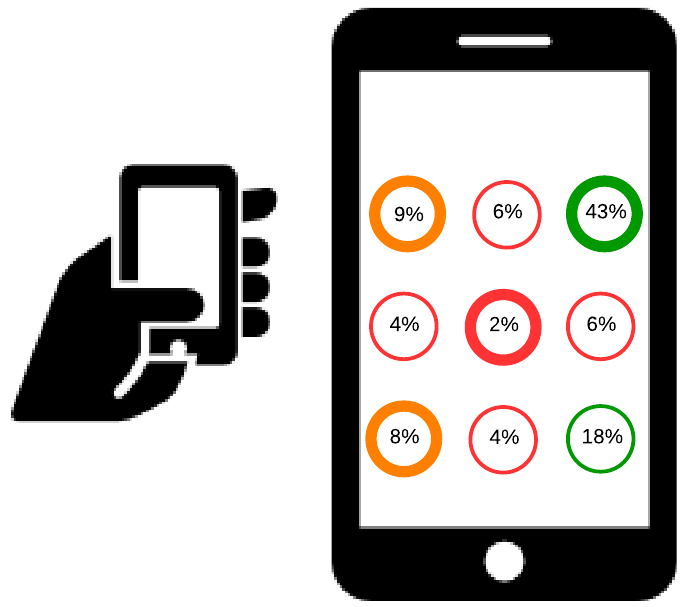
\includegraphics[scale=0.2]{pics/review/handednessLeft.png}
          }
          \subfigure{
            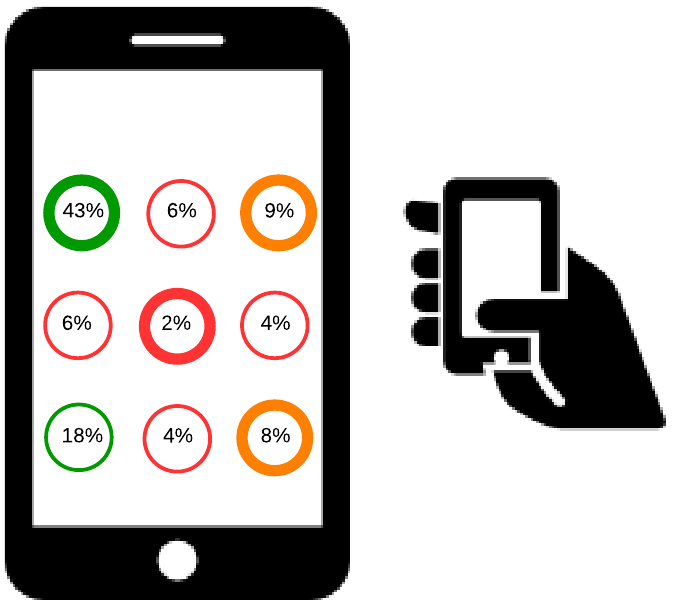
\includegraphics[scale=0.2]{pics/review/handednessRight.png}
          }
          \caption[Likely chosen initial starting point and handedness]{Likely chosen initial starting point \cite{Uellenbeck} and handedness}
          \label{fig:handedness}
        \end{figure}

      \subsection*{Nationality} 
      The nationality of users is often used in research on graphical passwords. When asking a person about their PIN code, a nationality can be used to find likely numbers to appear because some cultures associates a number with a historical or religious event. In a research on the {\it PassFace}, the nationality of the participants was proven to be valuable because people tended to choose faces from the same race and nationality. In this research, it is uncertain how much this information will help to prove any connection between nationality and users choice in patterns. Properties like language preference and reading/writing orientation look more promising for this research. However, the nationality is a data property that are useful when getting an overview of the population.

      \subsection*{Reading and writing orientation}
      In different cultures, there is a difference in the reading and writing orientation. Cultures of Europe and America usually write and read horizontally from left to right, but there are other cultures that do otherwise. Figure \ref{fig:orientation} illustrates three different ways of reading and writing. Traditionally, Chinese, Japanese, and Korean are writing text vertically in columns from top to bottom, from right to left. Another writing orientation is horizontal from right to left used in Arabic speaking countries. Today, the vertical orientation from top to bottom is often in a horizontal way due to the influence of English and the increased computerized typesetting, but both ways are still in use. There is research that have reported that the writing orientation are affecting the visual attention and memory \cite{Chan}. They found that the reading orientation affected the way a person would memorize objects. They reported that English and Chinese speakers tended to remember an image that appeared in the top, left-hand side of the screen. The Taiwanese speakers in the study tended to remember images on the opposite side of the screen, the images on the upper-right side of the screen. An interesting aspect of the reading and writing orientation is to see if people from different cultures are choosing different patterns due to their writing orientation. 

        \begin{figure}[H]
          \centering
          \subfigure[Left-to-right]{
            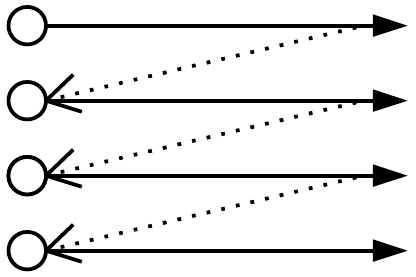
\includegraphics[scale=0.25]{pics/review/leftright.png}
          }
          \subfigure[Right-to-left]{
            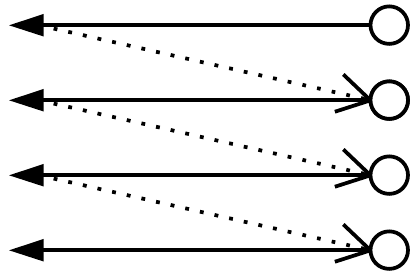
\includegraphics[scale=0.25]{pics/review/rightleft.png}
          }
          \subfigure[Top-to-bottom, left-to-right]{
            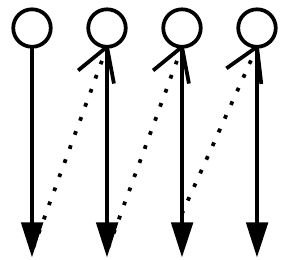
\includegraphics[scale=0.27]{pics/review/topbottom.png}
          }
          \caption{Reading and writing orientation}
          \label{fig:orientation}
        \end{figure}

      \subsection*{Profession and Occupation}
      The current profession of a person may say something about persons knowledge and background. When looking at profession, a person with a profession in IT may be more certain of the security aspects than people in other professions. It may cause bias in the data if people with enough knowledge of security overcompensate their choice of lock pattern because they want to prove their knowledge. Occupation is valuable information due to the knowledge level of the respondents. The occupation of the a respondent is simply if a person is a student, employed, not employed or retired.

      \subsection*{Finger, handsize, and screensize}
      When looking at the finger used when creating the pattern, it impacts the reachable areas on the smartphone. When interacting with a smartphone, the most common way is to either use the thumb or the forefinger. When combining this property with the screen size and the size of the hand, we might be able to predict the selection of patterns by eliminating areas that are harder to reach. In a book called {\it Designing Mobile Interfaces} \cite{Hoober}, they used an expression called the {\it thumb zone}. The Thumb Zone is the most comfortable area for a person to touch when holding a smartphone using one hand. Figure~\ref{fig:thumbZone} is showing the thumb zone where the green area is where the thumb can easily access. The orange and the red areas are part of the screen that is harder to reach. The thump zone can be used when looking at users choice of patterns a pattern that are easy to type can be more likely of being created. Smartphones today tends to get bigger and bigger in size. An interesting analysis could be done by looking at user's choice in patterns based on the size of their hands and size of the screen. By looking at a situation where a person with a small hand is interacting with a big screen, it may be hard to reach certain areas of the screen when holding the smartphone in one hand. Maybe a right-handed person with a small hand interacting with a large screen will not be able to reach the upper left corner? The situation are illustrated in Figure~\ref{fig:reachablePoints}.

        \begin{figure}[H]
          \centering
          \subfigure[Reachable points on screen]{
            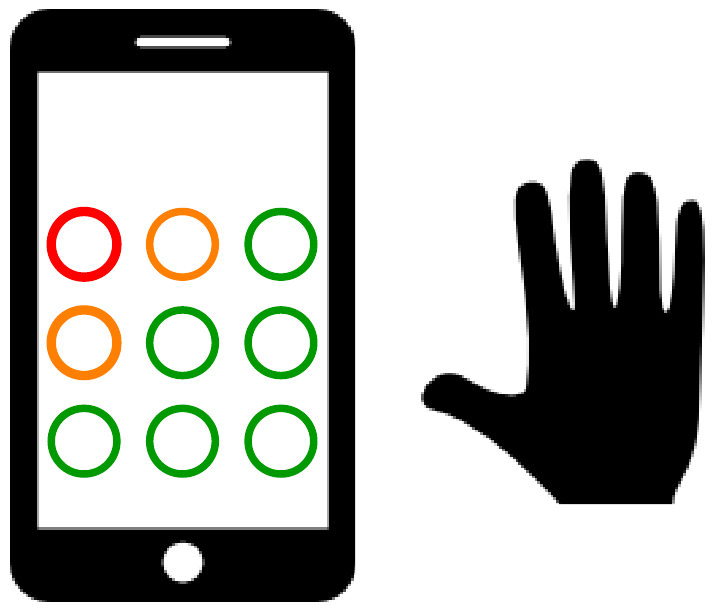
\includegraphics[scale=0.22]{pics/review/screenHand.png}
            \label{fig:reachablePoints}
          }
          \hspace{1.0cm}
          \subfigure[The thumb zone]{
            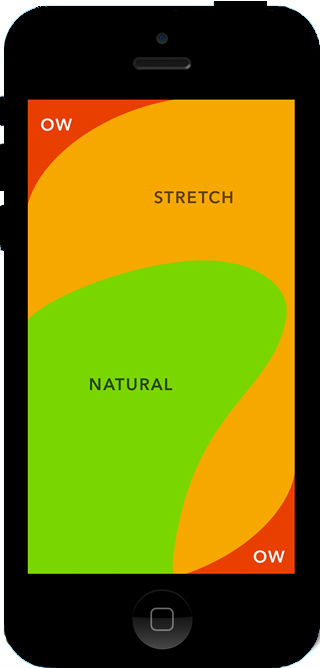
\includegraphics[scale=0.20]{pics/review/mobileScreen.jpg}
            \label{fig:thumbZone}
          }
        \end{figure}

      % \subsection*{Selection of Human Properties}
      % Based on the human properties review, not all of them have the same potential for being included in the data collection. First, the human properties have to have potential for getting interesting results. Second, the property are collected from a mobile survey, meaning that it have to be possible to collect the information based on a question. 

      % The handsize of a person and the finger used when creating the pattern is an interesting combination. The screensize is not directly a human property, but is included because is impacts the reachable areas on a mobile screen based corresponding to the handsize. The finger used can be directly asked for in the survey, while screensize and handsize are categorized as being subjective. When collecting handsize and screensize, the data collected needs to be further evaluated for its validity.

      % Nationality and reading and writing orientation are two properties closely related, and both properties are further included. Language preference will not be included in the survey as there are many languages. 

      % Profession and occupation is not easy to ask for as the number of professions are high as well as depending on where a person live. It is not easy to obtain any significant result as there are too many professions. Instead of collecting all professions, the experience with IT and security are included as it is relevant to the topic of research. 

      % Age and gender are information that are characteristic to have when analysing subgroups, as well as getting an overview of the entire population. 
      % Handedness 
  
  \section{Calculating the Sample Size} \label{sec:samplesize}

    It is essential to determine an appropriate sample size to be able to make any conclusions with the data. When a sample size is too big, it will lead to an unnecessary waste of time in this study due to the time frame of the thesis. On the other hand, if the sample size is too small, the results can not be considered to be used for statistical tests, and it might not be possible to come up with a reliable conclusion.

    When using known formulas for calculating the sample size, you need to know the population size, preferred margin of error, desired confidence interval, and the percentage of the population that is likely to answer. In this study, these parameters are hard to determine because of the non-probability sampling technique that are being selected for this study. For example, the targeted population size is hard to estimate because it includes all people with a smartphone worldwide. Because of the uncertainty connected to the sampling technique, there do not exist a known formula for calculating the sample size. We are not able to calculate the sample size by a known formula, but the sample size still needs to be decided based on my subjective meaning. The sample size is determined by what is achievable with the time frame available, as well as what I as a researcher think of as a good enough sample to ensure sufficient data for getting any results.

    The greater the accuracy required by my claim that my sample size represent the whole population adequately; the larger your sample size needs to be. Statisticians have produced tables that correlate population size against the sample size for the required level of confidence and accuracy. Table~\ref{tab:sampleSize} is a recommended sample size for using a survey (using 95\% confidence interval and +/- 3\% accuracy range) estimated by the targeted population size \cite{empiriske}. As stated in Table~\ref{tab:sampleSize}, the sample size does not increase at the same rate as the target population. When looking at all people that owns a mobile phone worldwide, we can argue that the targeted population size is greater than 1,000,000, and we, therefore, need a sample size of at least 1000. It would be desirable to get a sample size bigger than 1000, but due to the time frame of this research, a sample size of 1000 should me achieved.

      \begin{table}[H]
        \centering
        \begin{tabular}{| p{5cm} | p{5cm} |}
          \hline
          {\bf Target Population Size} & {\bf Required sample size} \\ \hline
          50 & 47 \\
          5000 & 760 \\ 
          100,000 & 888 \\
          900,000 & 895 \\ 
          $>$1,000,000 & 1000+ \\ \hline
        \end{tabular}
        \caption{Target population and sample size \cite{empiriske}}
        \label{tab:sampleSize}
      \end{table}

    Since the sampling size is quite high, and the survey is being distributed with a self-selection sampling strategy over the Internet, it is still important to provide some level of control of the respondents. Using a self-selection sampling technique implies that there is no control of who will answer the survey, hence likely that some subgroups will have a higher representation that others. In a situation where lacking respondents from a subgroup, it should be recruited more participants from the subgroup. However, when using such a strategy, it might introduce some bias because I would then influence the sample. Section \ref{sec:response} will look at some strategies for responses from different subgroups that may be underrepresented when using a self-selection sampling technique. 

  \section{Response Rate and Non-responses} \label{sec:response}

    The survey is distributed over the internet, making it difficult to maintain control over how many people are willing to respond and how many people from different subgroups that are reachable. To be able to achieve the amount of data needed for an analysis, a strategy are need if a subgroup are being underrepresented in the sample. Below, there are listed a strategy for collecting data from the different subgroups. The strategies are being included as a cause of some subgroups might being less willing to respond, or harder to reach, because they are outside the network of the people involved in this research.

    {\bf People with age of 60 or higher:} 
    People with the age over 60 may not own a smartphone or may be hard to reach for other reasons. It would be beneficial to find networks where containing a high representation of people with an age of 60 or higher. In Norway, there is a network called "Seniorweb." There is also a magazine called ``vi over 60''  for senior citizens with members with an age over 60. Both networks are possible to contact if there is a lack of respondents from this subgroup.

    {\bf People with a different field of interest than IT and security:} 
    The network of the people involved in this research is being overrepresented by people with a profession in IT and security. It is needed to find other networks to be able to reach out to other people with other jobs. For reaching out to people with other professions, it is a possibility to use the network from my family or directly contact a company in an another field. The university is a good start because of the high representation of different fields of study.

    {\bf People with a reading orientation from right-to-left:} 
    The primary reading orientation is from right-to-left, except some Arabic and Asian nationalities. My network does not include a high sample of people that have another reading and writing direction than my own. To reach out to other nationalities, NTNU is a possibility for getting help to distribute the survey to countries where NTNU have exchange programs. 
    
    {\bf People living in a different country than Norway:} 
    The sample should include respondents from different nationalities to obtain diversity in the sample. It is not easy to reach out to other countries if not having a big international network. NTNU has exchange students at the campus from different parts of the world. The preliminary work for this thesis was presented at a conference named Passwordscon. At the conference, many security interested people met at the conference are potential help for the distribution of the survey to other countries. 

    {\bf People that are left-handed:} 
    There is a significant higher percentage of people that are right-handed, meaning that there is a possibility of getting more responses from right-handed people. Selecting a strategy for this is hard because there is not a known official network for left-handed people. There is a possibility of using groups at Facebook like ``Left-Hander's Club.''
    